\documentclass{article}
\usepackage{xeCJK}
\usepackage{amsmath}
\usepackage{listings}
\usepackage{xcolor}
\setlength{\parindent}{0pt}
\renewcommand{\baselinestretch}{1.0}
\lstset{
	frame=tb, % draw a frame at the top and bottom of the code block
	showstringspaces=false, % don't mark spaces in strings
	numbers=left, % display line numbers on the left
	commentstyle=\color{green}, % comment color
	keywordstyle=\color{blue}, % keyword color
	stringstyle=\color{red} % string color
}
\usepackage[a4paper,left=20mm,right=20mm,top=15mm,bottom=15mm]{geometry}  

\title{AC自动机}
\author{MengChunlei}

\begin{document}
\maketitle
\section{题目描述}
给定一些串的集合$S=\{s_{1},s_{2},...,s_{m}\}$, 以及一个串$T$.问$T$包含了给定集合中的哪些串.这是$AC$自动机要解决的问题. \par
\section{结构描述}
算法的思路是首先为集合$S$建立AC自动机,然后在AC自动机上查询$T$.\par
AC自动机首先是一棵树.假设集合$S=\{i, he, his, she, hers\}$,那么对应的树为: \par
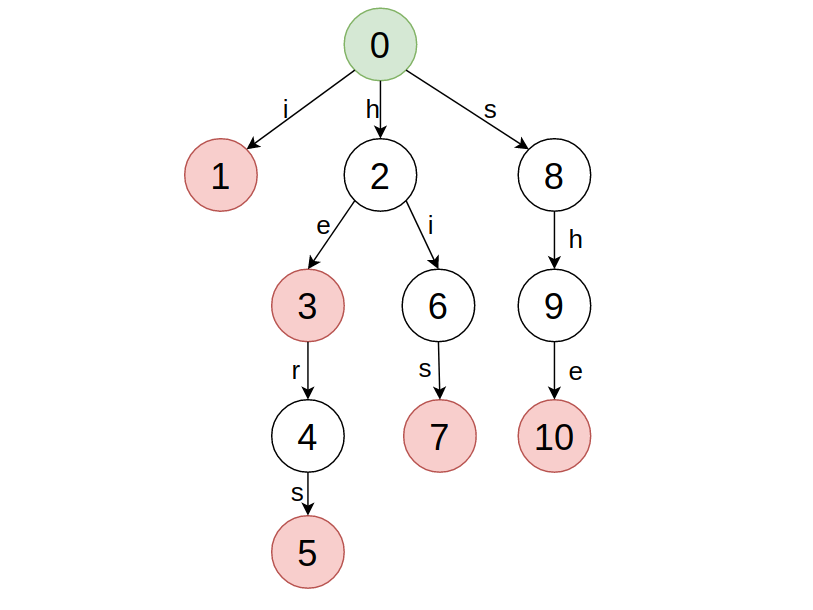
\includegraphics[scale=0.45]{pic1.png} \par
其中,绿色的0号节点为根节点,表示空串.其他每个节点代表的串为从根节点到当前节点经过的边上的字符组成的串,比如节点3代表he,节点6代表hi.红色的节点代表的串为集合$S$中的串.所以每个节点其实保存了每个字符对应的孩子节点,比如$E(2,i)=6$,表示在节点2表示的串后加上字符'i'所对应的新串的节点为6.\par
~\\
另外,每个节点还有一种边,叫做$fail$边,$fail$边到达的节点所表示的串是当前节点表示的串的最长后缀.在上面的例子中, 比如节点7代表的串为his, 可以发现,它的$fail$边会指向节点8, 因为不存在is的节点,只有s的节点8.如下图所示: \par
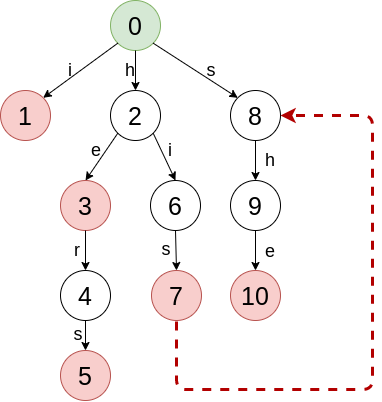
\includegraphics[scale=0.35]{pic2.png} \par
进而我们可以把所有的$fail$边都加上: \par
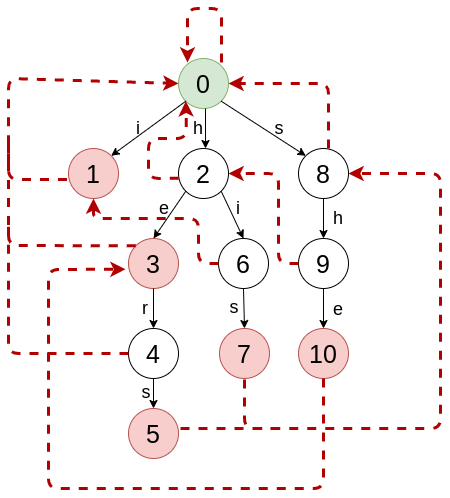
\includegraphics[scale=0.6]{pic3.png} \par
~\\
现在来总结下这个节点的数据结构: \par

\begin{lstlisting}[language=C++, caption={Node defination}]
struct Node {
  std::map<char, Node*> sons;
  Node* fail;
  int target_set_index; // The index word in S, -1 if not

  bool HasSon(char ch) const { return sons.count(ch) > 0; }
  const Node *GetSon(char ch) const { return sons.at(ch); }
  Node *GetSon(char ch) { return sons.at(ch); }
};
\end{lstlisting}

在这个节点的基础上,假设现在已经建立了给定$S$的AC自动机,那么查询$T$包含了$S$中的哪些的逻辑如下: \par

\begin{lstlisting}[language=C++, caption={Query}]
std::set<int> Query(const Node *root, const std::string &T) {
  std::set<int> result;
  const Node *curr = root;
  for (char ch : T) {
    const Node *son = root;
    do {
      if (curr->HasSon(ch)) {
        son = curr->GetSon(ch);
        break;
      }
      curr = curr->fail;
    } while (curr != root || curr->HasSon(ch));
    if (son->target_set_index >= 0) {
      result.insert(son->target_set_index);
    }
    curr = son;
  }
  return result;
}
\end{lstlisting}
下面来解释一下这个函数.第2行的$result$用来存储结果,即包含的目标串的编号.第3行设定当前节点为根节点,当前节点的含义是它表示的串是当前$T$的最长后缀.接下来这个主循环分两大部分,第一部分从第5行到第12行,是为了找到一个节点使得这个节点代表的串是$T$的当前前缀($T[0,i]$)的最长后缀.由于$curr$节点的串是$T[0,i-1]$的最长后缀,所以第7行,如果$curr$有一个孩子是$ch$,那么这个就节点就是$T[0,i]$的最长后缀,第8-9行设置并退出循环.否则第11行,$curr$跳转到它的$fail$节点, 因为它的$fail$节点的串是$curr$的最长后缀,如果这个节点有个$ch$的孩子,那么那个孩子节点就是目标,这样就进入了下一个循环.最后第12行结束的另一个条件,到达了根节点并且根节点没有为$ch$的孩子,那么说明没有非空节点的串是$T$的后缀,这时当前节点就是根节点.然后第二部分第13-16更新答案并重新设置$curr$. \par
~\\
下面给一个例子来模拟节点的跳转,假定$T=ushersheishis$ \par
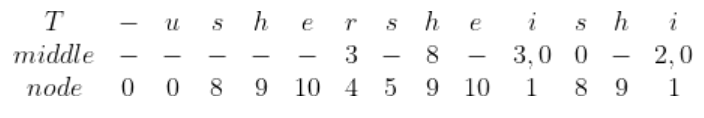
\includegraphics[scale=0.5]{pic4.png} \par

\section{构造过程}
分两部分,第一部分是插入字符串并建立孩子边,第二部分是建立$fail$边.第一部分比较简单,代码如下: \par
\begin{lstlisting}[language=C++, caption={Insert}]
void Insert(const std::string &s, int id, Node* root) {
  Node* curr = root;
  for (char ch : s) {
    if (!curr->HasSon(ch)) {
      Node* p = new Node;
      p->target_set_index = -1;
      curr->sons[ch] = p;
    }
    curr = curr->GetSon(ch);
  }
  curr->target_set_index = id;
}
\end{lstlisting}

第二部分是$fail$边的建立.这个可以按照$bfs$的过程从深度由小到大进行建立.首先,是根节点和深度为1的节点,因为这些节点的长度只有1,所以没有更短的串是它们的后缀了,只有空串,所以它们的$fail$都指向根节点. \par
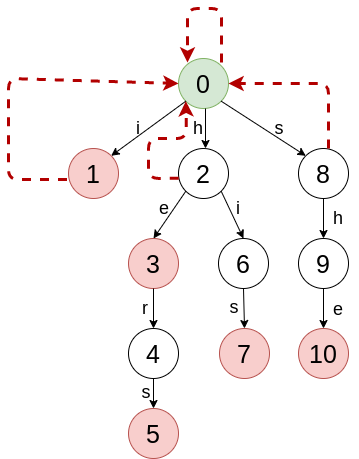
\includegraphics[scale=0.5]{pic5.png} \par

从深度为2开始,来分析一个节点$node$的$fail$应该是谁.假设$node$的父节点是$father$,并且$father$到$node$的边为字符$ch$.因为建立$fail$是按照深度递增进行的,所以$father$节点的$fail$指针已经建立好了.如果$father$的$fail$节点$q$有一个$ch$的孩子$p$,那么$p$就是$node$的$fail$节点.因为$q$是$father$的最长后缀.否则只需要沿着$q$的$fail$边一直向上找,直到找到一个节点$r$,使得$r$有一个$ch$的孩子$t$,那么$t$就是$node$的$fail$节点.具体的示意图如下所示: \par
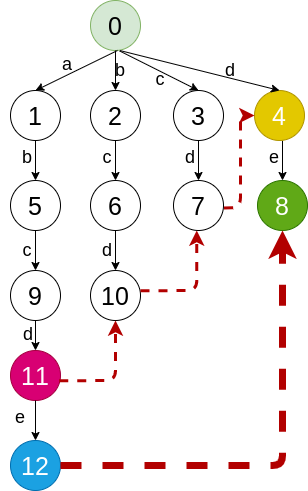
\includegraphics[scale=0.64]{pic6.png} \par
其中$node$节点是12,$father$节点是11, 最后沿着$fail$边,$11\rightarrow 10\rightarrow 7\rightarrow 4$, 最后找到节点4的时候,它有个$e$的孩子.所以12的$fail$节点为8. \par
下面是代码的实现: \par
\begin{lstlisting}[language=C++, caption={Build}]
void Build(Node *root) {
  std::queue<Node *> nodes;
  for (auto &e : root->sons) {
    e.second->fail = root;
    nodes.push(e.second);
  }
  while (!nodes.empty()) {
    Node *father = nodes.front();
    nodes.pop();
    for (auto &e : father->sons) {
      char ch = e.first;
      Node *node = e.second;
      Node *fail = father->fail;
      while (fail != root && !fail->HasSon(ch)) {
        fail = fail->fail;
      }
      if (fail->HasSon(ch)) {
        node->fail = fail->GetSon(ch);
      } else {
        node->fail = root;
      }
      nodes.push(node);
    }
  }
}

\end{lstlisting}
~\\
在上面的代码中的第14行寻找合适的$fail$节点的时候,这个循环可能会执行很多次,从而导致时间复杂度变大.有一个解决的办法采用了空间换时间的概念,代码如下面所示.它的改进在于,如果在插入完集合$S$中的字符串后,如果一个节点$p$没有孩子为$ch$的节点,那么将强行增加一条这样的边,它到达的节点所代表的串为节点$p$代表的串加上字符$ch$所得到的新串的最长后缀.如下面的代码的第32行所示 \par

\begin{lstlisting}[language=C++, caption={FastBuild}]
struct Node {
  std::vector<Node *> sons;
  Node *fail;
  int target_set_index;

  Node() : sons(26, nullptr), fail(nullptr), target_set_index(01) {}

  bool HasSon(char ch) const { return sons[ch - 'a'] != nullptr; }
  Node *GetSon(char ch) { return sons.at(ch - 'a'); }
};

void FastBuild(Node *root) {
  std::queue<Node *> nodes;
  for (char ch = 'a'; ch <= 'z'; ++ch) {
    if (!root->HasSon(ch)) {
      root->sons[ch - 'a'] = root;
    } else {
      Node *son = root->GetSon(ch);
      son->fail = root;
      nodes.push(son);
    }
  }
  while (!nodes.empty()) {
    Node *father = nodes.front();
    nodes.pop();
    for (char ch = 'a'; ch <= 'z'; ++ch) {
      if (father->HasSon(ch)) {
        Node *son = father->GetSon(ch);
        son->fail = father->fail->GetSon(ch);
        nodes.push(son);
      } else {
        father->sons[ch - 'a'] = father->fail->GetSon(ch);
      }
    }
  }
}

\end{lstlisting}

\end{document}
